\documentclass{standalone}
\usepackage{tikz}
\usetikzlibrary{shapes,arrows,positioning}
\begin{document}
 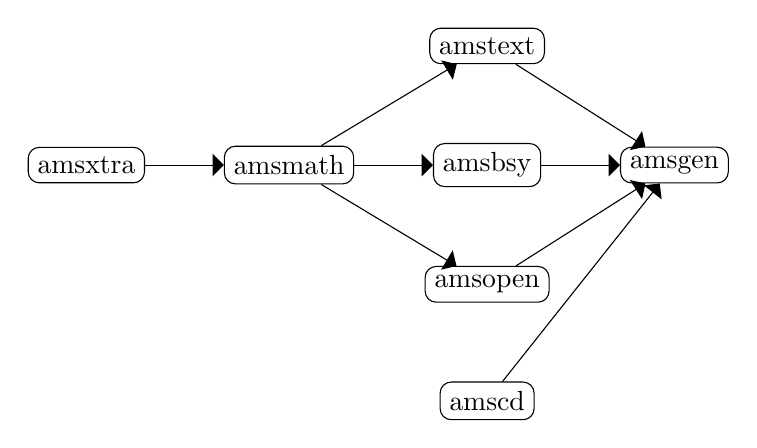
\begin{tikzpicture}
 \tikzset{main node/.style={rectangle, draw,
 		text centered, rounded corners}, }
 \tikzset{internal node/.style={rectangle, draw,dotted,
 		text centered, rounded corners}, }
 \tikzset{driver node/.style={ellipse, draw,dashed,
 		text centered}, }
 \tikzset{formato node/.style={rectangle, draw,dotted,
 		text centered}, }
 \tikzset{cfg node/.style={minimum size=1cm}, }
 \tikzset{linea/.style={-triangle 90},}
 \node[main node] (1) {amsxtra};
 \node[main node] (2) [right =of 1] {amsmath};
 \node[main node] (5) [right =of 2] {amsbsy};
 \node[main node] (6) [below =of 5] {amsopen};
 \node[main node] (4) [above =of 5] {amstext};
 \node[main node] (3) [below =of 6] {amscd};
 \node[main node] (7) [right =of 5] {amsgen};
 \foreach \x /\y in{1/2,2/4,2/5,2/6,4/7,5/7,6/7,3/7}
 \path[linea] (\x) edge node {} (\y);
 %% 
 \end{tikzpicture}
\end{document}